\documentclass[a4paper,12pt]{article}

\usepackage[utf8x]{inputenc}
\usepackage[T1]{fontenc}
\usepackage{lmodern}

\usepackage{amsmath}
\usepackage{amssymb} % math symbols
\usepackage{geometry}
\usepackage{a4wide}
\usepackage{enumerate}
\usepackage{xcolor}
\usepackage{listings}
\usepackage{graphicx}
\usepackage{lastpage}

\usepackage{hyperref}

\usepackage{fancyhdr}
\pagestyle{fancy}
\fancyhead{}
\fancyfoot{}

\renewcommand{\contentsname}{Summary}

\lhead{Axel Angel \& Luca La Spada \& Guillaume Martres}
\rhead{Big data}
\rfoot{Page \thepage\ of \pageref{LastPage}}
\lfoot{\today}

\begin{document}
%\begin{titlepage}
\begin{center}
\sffamily


\null\vspace{2cm}
{\Huge CodecWatch \\[12pt] A multi-encoder comparator ?} \\[24pt]
\textcolor{gray}{\small{Big Data \\ École Polytechnique Fédérale de Lausanne}}

\hbox{\hspace{-20ex}

\includegraphics[width=19.5cm]{figures/White}}

\vfill

\begin{tabular} {cc}
\parbox{0.3\textwidth}{
\includegraphics[width=4cm]{figures/epfl}}
&
\parbox{0.7\textwidth}{%
	by \\ [4pt]
	\hspace{3em} Martres Guillaume (203085)\\
	\hspace{3em} Angel Axel (201284)\\
	\hspace{3em} La Spada Luca (193276)\\[9pt]
\small

Lausanne, EPFL, \today}
\end{tabular}
\end{center}
\vspace{2cm}
\end{titlepage}

\tableofcontents

\newpage

\section{Introduction}
% Project presentation and goals
New and emerging video codec standards like
HEVC/H.265~\footnote{\url{http://hevc.info/}} (MPEG standard),
VP9~\footnote{\url{http://www.webmproject.org/vp9/}} (open, royalty-free codec
developed by Google) or Daala~\footnote{\url{http://xiph.org/daala}} (research
project developed in the open by Mozilla) have caused a great increase of
activity around open source video encoders for these formats. The main challenge
of any encoder is to provide the greatest visual quality at acceptable file size
and encoding speed. This means that all these projects must measure their output
quality and compare it with the state of the art. It would be a great boost to
productivity for developers if an open source project to compare and track the
quality of these evolving encoders existed. This is the goal of CodecWatch,
which provides the following functionalities:
\begin{itemize}
\item Do nightly encode of a standard set of video clips using the latest git
revision of various open source encoders, at various bitrates.
\item Display in graph forms various metrics (like
PSNR~\footnote{\url{https://en.wikipedia.org/wiki/PSNR}} or
SSIM~\footnote{\url{https://en.wikipedia.org/wiki/SSIM}})
\item As quality metrics are only an approximation of the actual visual quality,
provide a way to compare the encoded videos side-by-side.
\end{itemize} Instead of starting from scratch, we implemented CodecWatch by
extending the existing open source encoding platform
OSCIED~\footnote{\url{https://github.com/davidfischer-ch/OSCIED}}.

\section{OSCIED description}
% Why we choose oscied, architecture summary
The goal of OSCIED is to provide a distributed cloud-powered platform to encode,
publish and manage distributed resources.  In practice it means that medias are
first uploaded to the platform, then multiple encoding jobs can be dispatched to
transformer machines and done in parallel.  The resulting medias are then
available in the platform for further processing or direct download by the
administrator.  Moreover these files can be published on any publisher machine
for public access.
% TODO: develop more
For more details, we invite the reader to consult the original paper by David
Fischer~\footnote{\url{https://github.com/davidfischer-ch/OSCIED/blob/master/docs/david/master_thesis/MA_DavidFischer_OSCIED_V2.pdf?raw=true}}.

% Explain we had to understand how OSCIED works, architecture complexity, it's enormous

\section{Deployment}
\subsection{OSCIED}
% what OSCIED provides to deploy, locally works fine
As the goal of OSCIED is to distribute computer resources across multiple
machines, the platform provides high-level scripts to deploy the different roles
locally or to a cloud provider.  Behind the scene OSCIED uses juju, a
provisioning and deployment tool that supports major cloud providers.  We won't
describe in detail how juju works but basically it is made of two parts: the
internals capable of interfacing with the cloud APIs and lots of
role-specific files (charms).  The charms are in fact description files which
tells the system how to deploy the different roles: package dependencies and how
to startup the services.  For example the webui of OSCIED needs a web server
thus the webui charm will tell juju to install Apache with PHP and setup the web
files in the right directory.

We first began to deploy a new instance of OSCIED with all roles locally on our
server at EPFL, each role inside its own LXC (linux container).  This involved
numerous bug fixes to OSCIED which where then merged upstream, see
\url{https://github.com/ebu/OSCIED/pulls?direction=desc&page=1&sort=created&state=closed},
\url{https://github.com/davidfischer-ch/OSCIED/pulls?direction=desc&page=1&sort=created&state=closed}
and
\url{https://github.com/davidfischer-ch/pytoolbox/pulls?direction=desc&page=1&sort=created&state=closed}.

\subsection{Provisioning on Microsoft Azure}
As video encoding is a very CPU intensive task, we had planned to use our
provided Azure instances to increase the number of videos and encoders we could
demonstrate our project on. Azure support required us to use a recent version of
Ubuntu and thus update OSCIED to account for changes in its dependencies (like
the removal of the -sameq argument from ffmpeg). This was completed
successfully, but unfortunately, we did not manage to properly deploy OSCIED on
Azure on time. This is due mostly to the quite complex and fragile scripts that
are normally used to deploy OSCIED and bugs in juju itself, like
\url{https://bugs.launchpad.net/juju-core/+bug/1316185} which we reported ourselves.

\section{Adaptations}
% modification we made, how we changed

\subsection{Code modification}
% TODO: Axel
To integrate our goals into OSCIED we decided to develop directly into the live
containers, we had direct feedback of our modifications.  Multiple roles were
affected: Orchestra, Transformer and Webui.  We needed to collect statistics
such as the video bitrate, quality measures such as PSNR/SSIM, media source such
as the git repository and commit, directly into the stored metadata of the media
at encoding time (these are pushed into the MongDB of the Orchestra role after
completion)

We had first to understand the internal implementation: hierarchy of files, the
classes and how they all work together.  This took us some time and finally we
were able to modify exactly what we wanted.  There were multiple obstacles due
to the dynamic nature of Python such as multiple level of indirections of the
API (callbacks) and the lack of type description, these components are lazily
coupled and they break only at runtime after a job.  Thus we had to debug our
code in live by looking at the logged files and iterate until we had what we
wanted.

First we decided to modify the Transformer code where the encoding process is
triggered after which the metadata are computed.  It is written in Python and
backed up by Celery, thus the call are all asynchronous and a callback is
called.  We modified the encoding target (ffmpeg) to collect more metadata
(called measures), these are computed by specialized programs of the Daala
project.

Secondly we had to modify Orchestra to accept these measures and put it as
regular metadata into the database. Some part of the code base is shared with
the Transformer and thus are written in Python but backed up by Flask (a light
server designed for serving APIs).

Thirdly the web interface Webui had to modified to display these informations,
this part is written in PHP.  Columns were added in the media pannel of the
interface in order to show the results of our tests and then for the final users
so he can compare numeric values directly.  As textual information is not
sufficient, we wrote a small API that serves these measures directly to a
separate interface with graphs.  We had to integrate our work with the PHP
framework of the Webui (called CodeIgniter), that is: register new routes and
ensure we provide a json output correctly to interpolate with Javascript (see
the next section).

\subsection{The Awesome CodecWatch Graph}
A new feature has been added: The Awesome CodecWatch Graph. It is a plot that shows you the evolution of the quality of different encoder on some specific video called sample. These results are retrieved from the OSCIED database. The graph gives you the possibility to filter the result by sample, by encoder, by metric. Moreover, you can set interval to retrieve only encoding that have been done in a specific range of dates.

The graph is coded principally in HTML, Javascript and CSS. It uses different Javascript plugins: Chosen~\footnote{\url{http://harvesthq.github.io/chosen/}} that change the default style of a multiselect in something with more hype, jQueryUI~\footnote{\url{http://jqueryui.com/}}, TimePicker~\footnote{\url{http://trentrichardson.com/examples/timepicker/}} that improves the default datepicker of jQueryUI in a more detailed one (you can set even the second), jQuery~\footnote{\url{http://jquery.com/}} and flotcharts~\footnote{\url{http://www.flotcharts.org/}} that is a jQuery plugin used to create plots.

An screenshot of a dummy graph is displayed in figure~\ref{fig:graph1}. The graph displays in the X-axis the bitrate and in the Y-axis the decibel of videos. If you pass your mouse over a point a tooltip appears with the exact values of the point.

\begin{figure}[!h]
	\centering
	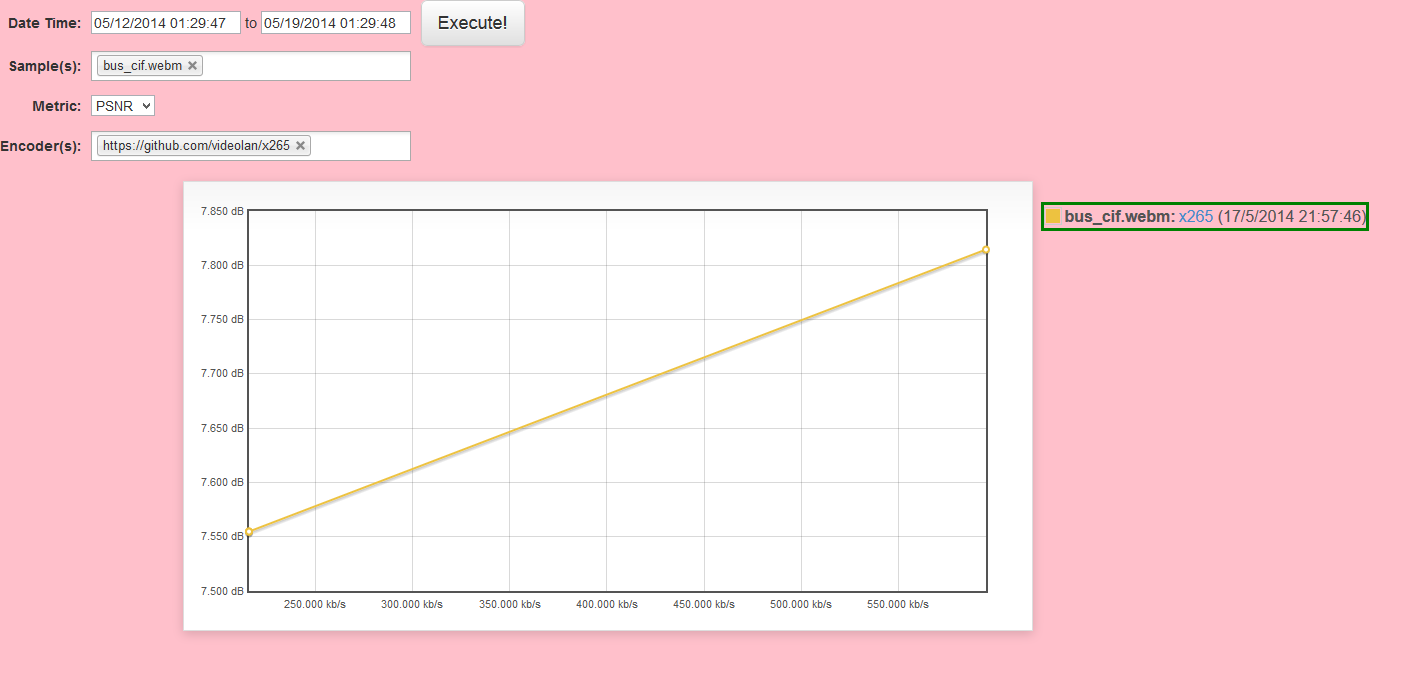
\includegraphics[width=1\textwidth]{figures/graph1.png}
	\caption{The Awesome CodecWatch Graph PROVISOIRE}
	\label{fig:graph1}
\end{figure}

\subsection{SplitView}
We included to the Webui of OSCIED the well-know visual comparator SplitView~\footnote{\url{https://github.com/smarter/splitview}}. Furthermore, we add a feature him. We have called it \emph{The Blind Test}. The blind test is all about the button that we can see in figure~\ref{fig:blindtest}. When we click it, the green square around the information about the videos becomes invisible and the two videos are swap with probability $0.5$. Thanks to this feature you loose completely the notion of which would be the best one based on his intrinsic value. When you reclick on the blind test button, the solution reappears.

\begin{figure}[!h]
	\centering
	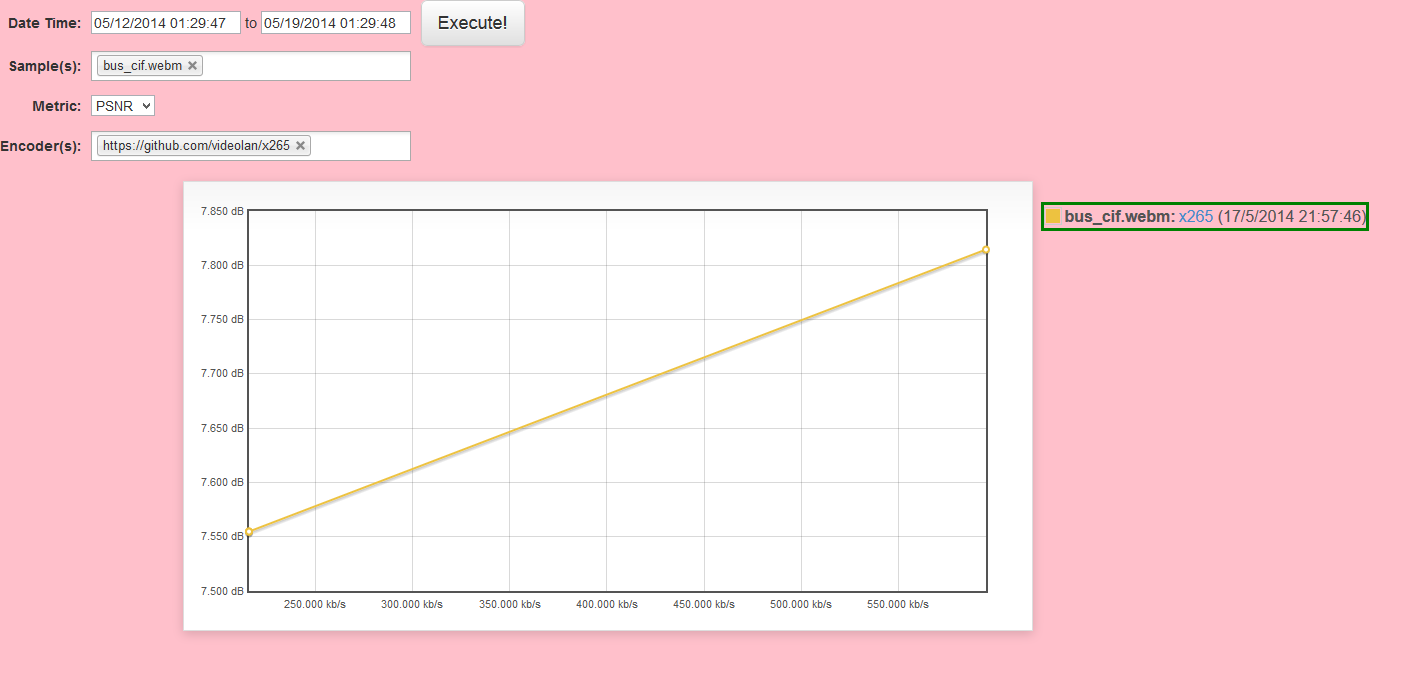
\includegraphics[width=1\textwidth]{figures/graph1.png}
	\caption{SplitView PROVISOIRE}
	\label{fig:graph1}
\end{figure}



% TODO: Luca

\section{Conclusion}
% what we made, sumup, how can be used and continued, improved
% what we did is useful, blabla

\end{document}
